Present the results of your analysis here.

\subsection{Explanation in dynamic graphs: a survey}


\begin{figure}[!h]
    \centering 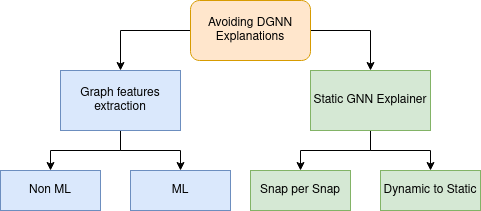
\includegraphics[width = 355pt]{Thesis_group_report_template_liris_en/Images/Avoiding DGNN Explainability Diagram.drawio.png}
    \caption{Avoiding dynamic GNN explainers} \label{fig:image}
    \label{other expl}
\end{figure}

1)static explainer working for Dynamic Graphs
2) Dynamic graphs changing graph into static one then static explainer
3)specific dy graphs explainer (table lit review 2) (not much anomaly detection...
4)graph features (topology,time) into classic ML
5)non ML --> stat, similarity in Time series,...

Figure~\ref{other expl} epxlain the figure...

+Table https://docs.google.com/document/d/1HVIT7x49c-3vlMisJMwkZ8TXNDjx-cXolEflYzA7QLw/edit explain...

\subsection{Application on Fraud transaction}

\subsubsection{Fraud detection}
DyHGN,xFraud,EvolveGCN
3 datasets

\subsubsection{Fraud explanation}
GNNExplainer+... (xFraud) static
XGBoost (DyHGN)

conclusion: use Perturbation methods better for 1) Anomaly detection 2) temporal (me lstm embeddings)
and/or similarity btw Time Series (DTW) similarity= explanation